
We consider a (matching) market of $k$ sellers and $k$ buyers, where $k$ is an integer, $k>0$. 
Each seller sells an item and the prices of the items are initially all zero. Buyer $i$ has valuation $k-i+1$ for the first item and valuation $0$ for every other item, as shown in the following diagram.

\vspace*{0.5cm}
\begin{tabular}{c r c c c}
    Buyers & \multicolumn{4}{c}{Valuations (for items $1$ to $k$)} \\
    \hline
    $x_1$ & $k,$ & $0,$ & $\ldots,$ & $0$ \\
    $x_2$ & $k-1,$ & $0,$ & $\ldots,$ & $0$ \\
    $\vdots$ & & & $\vdots$ \\
    $x_k$ & $1,$ & $0,$ & $\ldots,$ & $0$ \\
\end{tabular}

\noindent The sellers find the market-clearing prices using the procedure discussed in the lectures.
\begin{enumerate}
    \item[(a)] What are the prices of the sellers' items ($1^{st}$ item, $2^{nd}$ item, \ldots, $k^{th}$ item) when the market clears? Which buyer gets the $1^{st}$ item and at what price?  \hfill{\bf [3 marks]}\smallskip

    The $1^{st}$ item is sold at a price of $k - 1$.
    The $2^{nd}$ to $k^{th}$ items are sold at a price of $0$.

    Buyer $x_1$ gets the $1^{st}$ item at a price of $k - 1$.

    \item[(b)] Justify your answers to (a).  \hfill{\bf [6 marks]}\smallskip

    Let Algorithm 1 be the procedure for finding market-clearing prices as shown in the lectures, $Y$ be the set of items where item $y_i$ is sold at $p_i, 1 \leq i \leq k$, $X$ be the set of all buyers $x_j, 1 \leq j \leq k$, and $x_{j,i}$ be the valuation of item $i$ by buyer $j$.

    \begin{theorem}
        For $k$ items and $k$ buyers, the matching market with the above setup results in the market-clearing prices $(k - 1, 0, \dots, 0)$ for items $1, 2, ..., k$ using Algorithm 1.
    \end{theorem}

    \begin{proof}
        Direct proof on $k$.

        Applying Algorithm 1, the sellers' prices are initialised $p_i = 0$ for $1 \leq i \leq k$ (step 1).
        The preferred-seller graph is constructed as follows.

        Since all buyers have a non-zero valuation of the first item (and zero of the rest), and all items are initially sold for zero, the only preferred seller for each buyer is item 1.
        Thus, an edge $(p_1, x_j)$ is formed for $1 \leq j \leq k$ (step 2).

        \hfil
        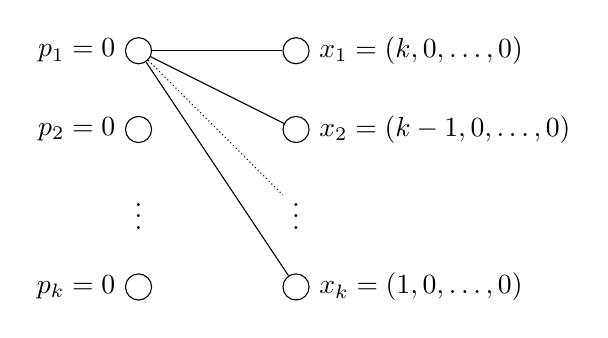
\begin{tikzpicture}[main/.style={circle,draw}]
            \node[main, label={left:$p_1 = 0$}] at (0, 2) (p1) {};
            \node[main, label={left:$p_2 = 0$}] (p2) [below of=p1] {};

            \node (pDots) [below of=p2] {\vdots};

            \node[main, label={left:$p_k = 0$}] (pn) [below of=pDots] {};

            \node[main, label={right:$x_1 = (k, 0, \dots, 0)$}] at (2, 2) (x1) {};
            \node[main, label={right:$x_2 = (k - 1, 0, \dots, 0)$}] (x2) [below of=x1] {};

            \node (xDots) [below of=x2] {\vdots};

            \node[main, label={right:$x_k = (1, 0, \dots, 0)$}] (xn) [below of=xDots] {};

            \draw(p1) -- (x1);
            \draw(p1) -- (x2);
            \draw[densely dotted](p1) -- (xDots);
            \draw(p1) -- (xn);
        \end{tikzpicture}
        \hfil

        This clearly does not form a perfect matching, so a constricted set $S$ of buyers is found (step 4).
        In this case, the neighbourhood of the constricted set $N(S)$ is $p_1$ no matter what constricted set $S$ is chosen (as $p_1$ is fully connected to the buyers and $p_i$ for $2 \leq i \leq k$ are disconnected).

        \begin{lemma}
            For the above setup, the neighbourhood $N(S)$ of any constricted set of buyers $S$ (at step 4 in Algorithm 1) is always $\{p_1\}$.
        \end{lemma}
        \begin{proof}
            Induction on the iterations of Algorithm 1 ($m$).

            \underline{Base case}:

            Let $m = 1$.

            For any $k$, the initial bipartite preferred-seller graph is the same as above.
            By inspection, $N(S) = {y_1}$, hence, for one iteration of Algorithm 1, the lemma holds.

            \underline{Inductive step}:

            Now assume the lemma holds true for the $m = r^{th}$ iteration.

            For step 2 of Algorithm 1, if there is a perfect matching, there cannot be a constricted set of buyers - in which case the algorithm terminates at step 3.
            Otherwise, at step 4, $p_1$ is the only vertex in $N(S)$ (by assumption of the truth of the lemma).

            $p_1$ is incremented by one in step 5.
            Given the lemma is assumed true up until this point, $p_1$ is the only price that has ever been incremented.
            This means that, before step 5 of iteration $r$, $p_1 = r - 1$ and after, $p_1 = r$, and $p_i = 0$ for $2 \leq i \leq k$.

            As there exists a zero price, no normalisation takes place in step 6 of Algorithm 1.
            This means that going into iteration $m = r + 1$, $p_1$ holds the value $r$.

            For step 2 of iteration $r + 1$, the preferred-seller graph is reconstructed.
            Again, if there is a perfect matching, the algorithm terminates at step 3.

            Observe the following three cases for a buyer $x_j$.

            \underline{Case 1}: \\
            When $p_1 < x_{j,1}$, $x_j$ is only interested in (and connects to) the first item.
            This is because buying $y_1$ gives the highest payoff compared to a payoff of zero from all the other items ($x_{j,1} - p_1 > 0$).

            \underline{Case 2}: \\
            When $p_1 = x_{j,1}$, $x_j$ is interested in (and connects to) all items (including the first).
            This is because buying the item $y_1$ has a payoff of zero - the same as all the other items ($x_{j,1} - p_1 = 0$).

            \underline{Case 3}: \\
            When $p_1 > x_{j,1}$, $x_j$ is interested in (and connects to) all items except the first.
            This is because the payoff for buying $y_1$ becomes negative, so they favour the next highest payoff which is zero for all the other items ($x_{j,1} - p_1 < 0$).


            Firstly consider the situation where $x_1$ finds its self in Case 1.
            This means means that $p_1 < x_{1, 1} \implies r + 1 < k$.
            Thus, $\exists j : 2 \leq j \leq k \implies r + 1 = x_{j, 1}$.
            The buyers can now be partitioned into two subsets.
            First, a subset who can win $y_1$, defined by $I = X - E = \{x_j : r + 1 \geq x_{j, 1}, 2 \leq j \leq k\}$.
            Second, a subset who can't win $y_1$, defined by $E = \{x_j : r + 1 < x_{j, 1}, 2 \leq j \leq k\}$.
            The first subset of length $a$ consists of the buyers in Case 1, the second subset of length $k - a$ consists of the buyers in Case 3.
            As it is established that buyers in Case 3 are fully connected to all items except the first, they form the complete bipartite graph $K_{k - 1, k - a}$.
            A subgraph of this is $K{a, a}$ since $n - a \leq k - 1$ which has a perfect matching.

            Suppose that $x_1$ found itself in Case 3 on the ${r + 1}^{th}$ iteration, $r + 1 > x_{1,1}$.
            By extension, all other buyers must also be in Case 3 -- overall $r + 1 > x_{j, 1}$ for $1 \leq j \leq k$.
            This means that no buyers are interested in item $y_1$ and hence no perfect matching can exist.
            Because of this, $S = X$ and $N(S) = Y - \{y_1\}$.

            At step 6 in Algorithm 1, $p_i = p_i + 1$ for $2 \leq i \leq k$ giving $\min{p_i} = 1$.
            This means that on the next iteration, all selling prices are reduced by 1, returning it to the same state as in iteration $r$.
            
            As this results in an infinite loop, the algorithm should never enter the state where $p_i > x_{1,1}$.
            For that to happen it would need to pass through the situation where $x_1$ finds its self in Case 2 ($p_1 = r + 1 = x_{1,1}$).
            This would also mean that all other buyers are in Case 3 ($r + 1 > x_{j, 1}$ for $2 \leq j \leq k$).
            This situation would also not occur because a perfect matching would have been found, terminating the algorithm at step 3.

            Because of this, continuation to step 4 of the algorithm means that $x_1$ must be (and other consecutive buyers might be) in Case 1, there is exactly one buyer in Case 2, and the rest are in Case 3.
            As such, item $y_1$ must be connected to all buyers in Case 1 (including at minimum $x_1$) and the one buyer in Case 2.
            Trivially, all buyers in Case 3 (those in the second subset) form a complete bipartite graph with all items except for the first.
            Furthermore, the second subset (buyers in Case 1 and the buyer in Case 2) must have a size at least $2$.
            If the size is $2$, there would exist a perfect matching and so the algorithm would have terminated.
            Hence, since the size must be greater than $2$, there is a subset $S$ of at least $2$ buyers in Case 1 which are only connected to item $y_1$.
            Finally, this shows that, for iteration $m = r + 1$, $S$ (and any subset of $S, |S| > 1$) forms the only constricted set with neighbourhood $N(S) = \{y_1\}$.
        \end{proof}

        Using Lemma 0.2, at step 5, Algorithm 1 only ever increments $p_1$ (because $y_1$ is the only item in $N(S)$ and $S$, and its subsets, form the only constricted set).
        Combining this with the additional remarks in Lemma 0.2, Algorithm 1 must therefore increment $p_1$ at each iteration until $x_2$ switches to Case 2, leaving a size of 2 for the first set (from Lemma 0.2), making it no longer a constricted set.
        
        Because $p_1$ is incremented by one each iteration, all other item prices remain 0, and $x_{1, 1} > p_1, x_{2, 1} = p_1$, it is necessary that $p_1 = k - 1$ and $p_i = 0, 0 < i \leq k$.
        This will result in the preferred-seller graph below.

        \hfil
        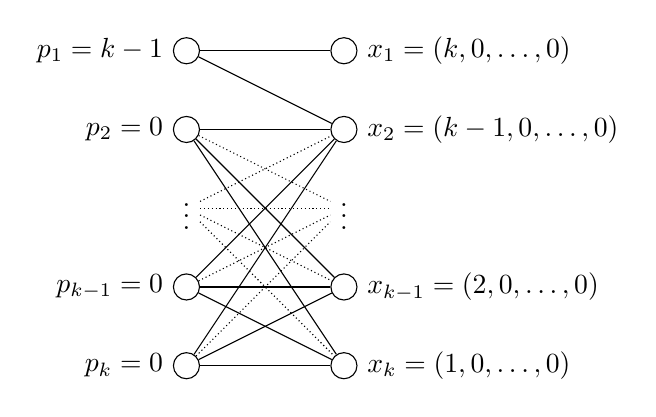
\begin{tikzpicture}[main/.style={circle,draw}]
            \node[main, label={left:$p_1 = k - 1$}] at (0, 2) (p1) {};
            \node[main, label={left:$p_2 = 0$}] (p2) [below of=p1] {};

            \node (pDots) [below of=p2] {\vdots};

            \node[main, label={left:$p_{k - 1} = 0$}] (pn1) [below of=pDots] {};
            \node[main, label={left:$p_k = 0$}] (pn) [below of=pn1] {};

            \node[main, label={right:$x_1 = (k, 0, \dots, 0)$}] at (2, 2) (x1) {};
            \node[main, label={right:$x_2 = (k - 1, 0, \dots, 0)$}] (x2) [below of=x1] {};

            \node (xDots) [below of=x2] {\vdots};

            \node[main, label={right:$x_{k - 1} = (2, 0, \dots, 0)$}] (xn1) [below of=xDots] {};
            \node[main, label={right:$x_k = (1, 0, \dots, 0)$}] (xn) [below of=xn1] {};

            \draw(p1) -- (x1);
            \draw(p1) -- (x2);

            \draw(p2) -- (x2);
            \draw[densely dotted](p2) -- (xDots);
            \draw(p2) -- (xn1);
            \draw(p2) -- (xn);

            \draw[densely dotted](pDots) -- (x2);
            \draw[densely dotted](pDots) -- (xDots);
            \draw[densely dotted](pDots) -- (xn1);
            \draw[densely dotted](pDots) -- (xn);

            \draw(pn1) -- (x2);
            \draw[densely dotted](pn1) -- (xDots);
            \draw(pn1) -- (xn1);
            \draw(pn1) -- (xn);

            \draw(pn) -- (x2);
            \draw[densely dotted](pn) -- (xDots);
            \draw(pn) -- (xn1);
            \draw(pn) -- (xn);
        \end{tikzpicture}
        \hfil

        Removing the vertices for seller $y_1$ and buyer $x_1$ yields the complete bipartite graph $K_{k - 1,k - 1}$.
        Hence, at step 2, Algorithm 1 now terminates because there is a clear parallel matching between $x_i$ and $y_i$ for $1 \leq i \leq k$.
        Indeed, the final item prices are $(y_1, y_2, \cdots, y_k) = (k - 1, 0, \cdots, 0)$ as required.

    \end{proof}

    \item[(c)] Which kind of auction does the construction of market-clearing prices procedure implement in this case?  \hfill{\bf [3 marks]}\smallskip

    As the winner of item $1$ is the buyer ($x_1$ in this case) who values it the highest.
    They pay the valuation of item $1$ by the second highest buyer ($k - 1$ in this case). 
    Thus, the construction of market-clearing prices implements a second-price (Vickrey) auction for item 1 in this case.

\end{enumerate}
